\section{Introduction}
\begin{frame}{\textbf{G}lobal \textbf{N}avigation \textbf{S}atellite \textbf{S}ystem}
    \begin{itemize}
        \item \textbf{GNSS} has been successfully applied in many fields:
    \end{itemize}

    \begin{figure}[!htb]
        \centering
        \begin{subfigure}[b]{0.3\textwidth}
            \centering
            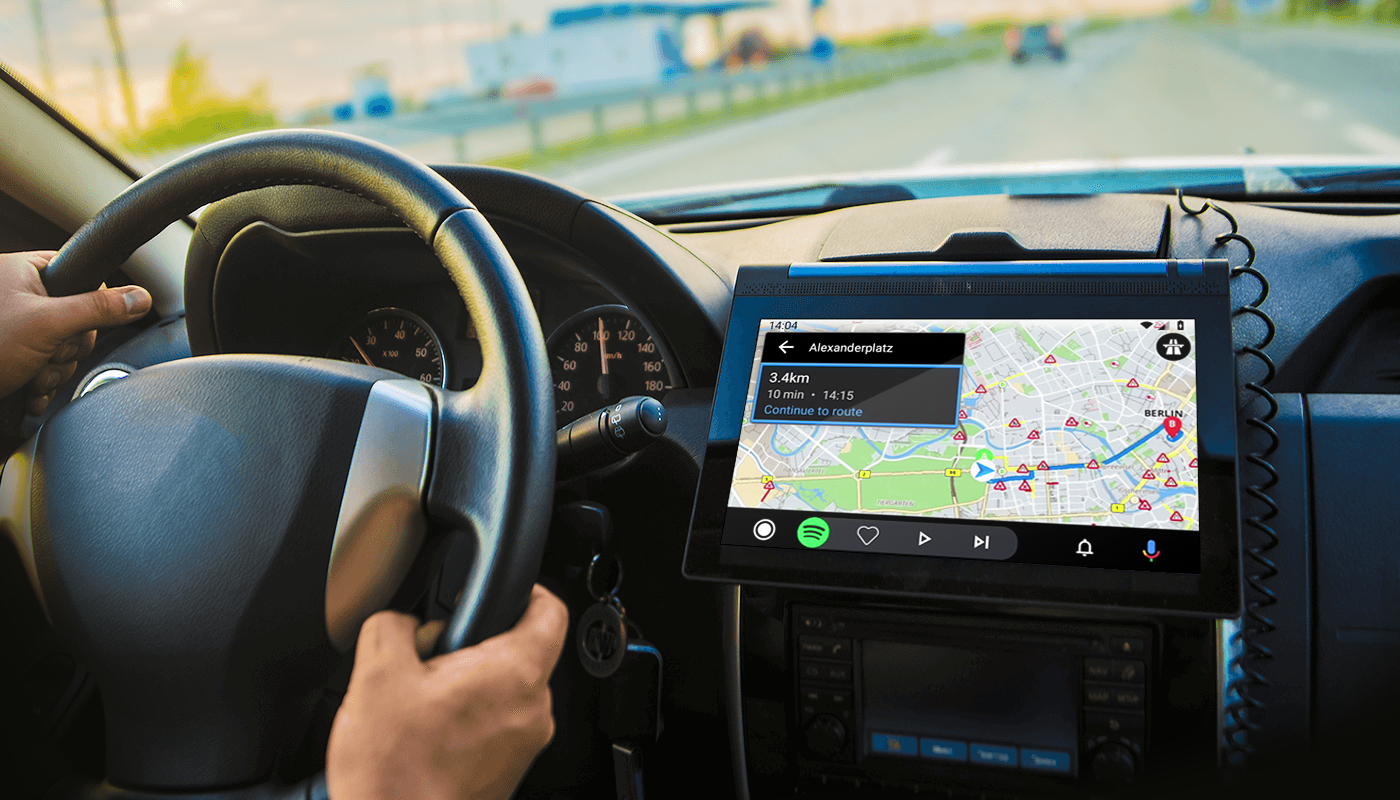
\includegraphics[width=\linewidth]{images/carnav.png}
            \caption{Car navigation}
            \label{fig:carnav}
        \end{subfigure}
        \hfill
        \begin{subfigure}[b]{0.3\textwidth}
            \centering
            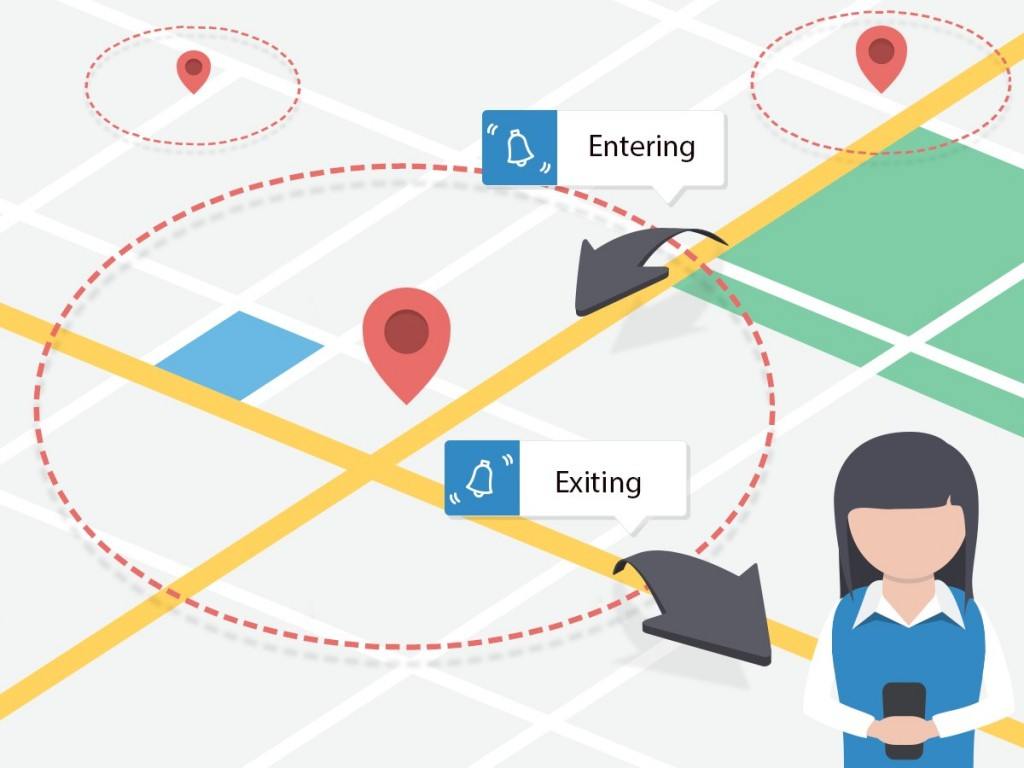
\includegraphics[width=\linewidth]{images/geofencing.jpg}
            \caption{Geofencing}
            \label{fig:geofencing}
        \end{subfigure}
        \hfill
        \begin{subfigure}[b]{0.3\textwidth}
            \centering
            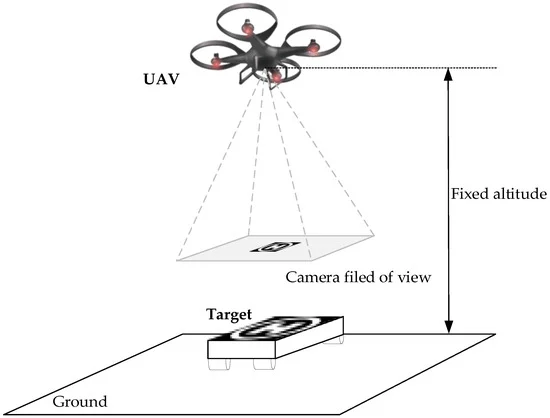
\includegraphics[width=\linewidth]{images/target.jpg}
            \caption{Target tracking}
            \label{fig:target}
        \end{subfigure}
           \caption{Some examples of application}
           \label{gnss}
    \end{figure}

    \begin{itemize}   
        \item It's \textbf{difficult to use} for inside location: \textbf{signal} is \textit{blocked} by buildings, trees, obstacles, ...
    \end{itemize}
\end{frame}

\begin{frame}{Indoor localization}
    \begin{itemize}
        \item It's even more \textbf{challenging}:
            \begin{itemize}
                \item Indoor spaces are more \textbf{complicated} in terms of \textit{layout}, \textit{topology}, \textit{space constraint};\item Indoor applications need more \textbf{accuracy}.
            \end{itemize}
        \item Multiple systems have been proposed in recent years:
        \end{itemize}
    
        \begin{figure}[!htb]
            \centering
            \begin{subfigure}[t]{0.24\textwidth}
                \centering
                
\includegraphics[width=\linewidth]{images/wifi.png}
                \caption{WiFi}
                \label{fig:wifi}
            \end{subfigure}
            \hfill
            \begin{subfigure}[t]{0.24\textwidth}
                \centering
                
\includegraphics[width=\linewidth]{images/zigbee.png}
                \caption{Zigbee}
                \label{fig:zigbee}
            \end{subfigure}
            \hfill
            \begin{subfigure}[t]{0.24\textwidth}
                \centering
                
\includegraphics[width=\linewidth]{images/bluetooth.png}
                \caption{Bluetooth}
                \label{fig:bluetooth}
            \end{subfigure}
            \hfill
            \begin{subfigure}[t]{0.24\textwidth}
                \centering
                
\includegraphics[width=\linewidth]{images/uwb.jpg}
                \caption{Ultra-wideband}
                \label{fig:uwb}
            \end{subfigure}
               \caption{Some examples of indoor localization systems}
               \label{indoor}
        \end{figure}
    
        \begin{itemize}
        \item Each technique has \textbf{drawbacks} in terms of accuracy, cost coverage, complexity and applicability.
    \end{itemize}
\end{frame}

% \begin{frame}{Hybrid methods}
%     \greent{PRO}

%     \begin{itemize}
%         \item Used to reach higher accuracy with relatively low cost.
%     \end{itemize}

%     \vspace{10pt}
%     \redt{CON}

%     \begin{itemize}
%         \item The required infrastructures may not be available in many environments or at a high cost.
%     \end{itemize}
% \end{frame}

% \begin{frame}{Spatial knowledge}
%     \begin{itemize}
%         \item Available in many scenarios;
%         \item It's used to assist localization without additional costs;
%         \item Helpful for calibrating the localization error.
%     \end{itemize}
% \end{frame}

\begin{frame}{Landmark}
    \begin{block}{Definition of \textbf{landmark}}
        A \textbf{landmark} is generally defined in the field of linguistics and cognitive science as everything that stands out of the background.
    \end{block}

    In the context of indoor localization, a landmark is 
    \begin{block}{Definition of \textbf{landmark} for indoor localization}
        A location point where at least one sensor presents a distinctive, stable  and identifiable pattern in the reading. Points are typically naturally distributed in indoor environments.
    \end{block}
\end{frame}


\begin{frame}
    \greent{PROS}
 
    \begin{itemize}
        \item Location points are naturally distributed in indoor environments;\item So $\rightarrow$ localization error easy to bound if combined;\item No extra cost required.
    \end{itemize}

    \redt{CONS}
    \begin{itemize}
        \item Economically or/and computationally expensive;
        \item Systems that use laser scanner and/ora cameras to do so are not suitable for indo pedestrian localization;
        \item Performances rely highly on the completeness of landmarks;
        \item A mismatch of landmarks causes large localization errors (= failure of localization).
    \end{itemize}
\end{frame}

\begin{frame}{LG-Loc}
    \begin{block}{Landmark-Guided Localization}
        It's a novel graph-based indoor localization method for smartphones
    \end{block}

    Compared with existing landmark-based localization methods:
    \begin{itemize}
        \item Computationally efficient;
        \item Handles incomplete landmarks;
        \item It uses landmarks to guide the localization process.
    \end{itemize}

    \begin{block}{Landmark graph}
        It's a directed graph where nodes are landmarks and edges are accessible paths with heading information
    \end{block}
\end{frame}

\begin{frame}{LG-Loc $\sim$ Phases}
    This method consists of two phases:

    \begin{enumerate}
        \item \textit{offline}: data from several smartphones sensors are collected. With these data th initial landmark graph is constructed. We update the landmark graph by adding more landmarks;
        \item \textit{online}: newly collected data are used for location initialization, estimation and calibration.
    \end{enumerate} 

    The initial location is inferred by a Hidden Markov model-based method and the location is regularly calibrated by matching the detected landmark with those in the landmark graph. 
\end{frame}

\begin{frame}{Challenges}
    \begin{enumerate}
        \item Infer the initial location without manual input;
        \item Recognize landmarks satisfying;
        \item Deal with a landmark association issue and missing landmarks.
    \end{enumerate}
\end{frame}